% vim: ts=2 sw=2 et tw=78 spell spelllang=en:
\section{Conservation Laws}

\begin{defn}[Conservation law]
  A \emph{conservation law} is a Cauchy problem of the form
  \begin{equation} \label{eqn:conservation-law}
    u_y + \partial_x f(u) = 0,
  \end{equation}
  for a given \emph{flux function} $f: \mathbb{R} \to \mathbb{R}$. An equivalent
  formulation is $u_y + c(u) u_x = 0$ with $c(u) = f'(u)$.
\end{defn}

\begin{defn}[Critical Time]
  Of an initial value (Cauchy) problem with conservation law
  \[
    \begin{cases}
      u_y + c(u) u_x = 0, & (x,y) \in \mathbb{R}\times(0,\infty), \\
      u(x, 0) = u_0(x), & x \in \mathbb{R},
    \end{cases}
  \]
  where $c, u_0 \in C^1(\mathbb{R})$ and such that $c \circ u_0 : \mathbb{R}
  \to \mathbb{R}$ is bounded and has bounded derivative, we interpret $y$ as
  being a ``time variable''. The \emph{critical time}
  \[
    y_c = \inf \left\{
      \frac{-1}{\alpha(s)}:
      s \in \mathbb{R}, \alpha(s) < 0
      \right\}
  \]
  where $\alpha(s) = \partial_s \bigl( c \circ u_0(s) \bigr) =
  c'(u_0(s))u_0'(s)$, is the time at which the solution is no longer smooth.
  If $\alpha(s) \geq 0$ for all $s \in \mathbb{R}$, we set by convention $y_c
  = \infty$.
\end{defn}
Therefore, the PDE has a unique solution in the interval $[0, y_c)$,
and $u$ satisfies the implicit equation
\[
  u(x,y) = u_0(x - c(u)y).
\]
Note that there can be multiple critical times, the infimum above only takes
the first. I.e. there could be a smooth solution solution after the critical
time, until a new critical time is reached.

\subsection{Weak solution}

\begin{defn}[Integral of a conservation law]
  Integrating \eqref{eqn:conservation-law} first wrt $x$ (space) then $y$
  (time) over an interval $X \times Y = [a,b)\times[y_1, y_2)$ results in
  \begin{align}
    \int_X u(x, y_2) &- u(x, y_1) \,dx \nonumber \\
    &= - \int_Y f(u(b,y)) - f(u(a,y)) \, dy.
    \label{eqn:conservation-law-int}
  \end{align}
\end{defn}

This is the \emph{integral formulation} of the conservation law, since if $u$
solves the conservation law \eqref{eqn:conservation-law} it also solves
\eqref{eqn:conservation-law-int}. However, because the integral is less
restrictive than the derivative and allows for discontinuities in the
solution, a solution to \eqref{eqn:conservation-law-int} may not be a solution
of \eqref{eqn:conservation-law}, it might be a \emph{weak solution}.

\begin{defn}[Weak solution and shocks]
  $u$ is a \emph{weak solution} on $D = \bigcup^n_{i=1} D_i$ if $u$ satisfies
  the PDE \eqref{eqn:conservation-law} in each $D_i$ for $i=1,\ldots,n$ and
  the integral form \eqref{eqn:conservation-law-int} on $D$. The boundaries
  between the regions $D_i$ are curves called \emph{shocks}.
\end{defn}

\begin{figure}
  \centering
  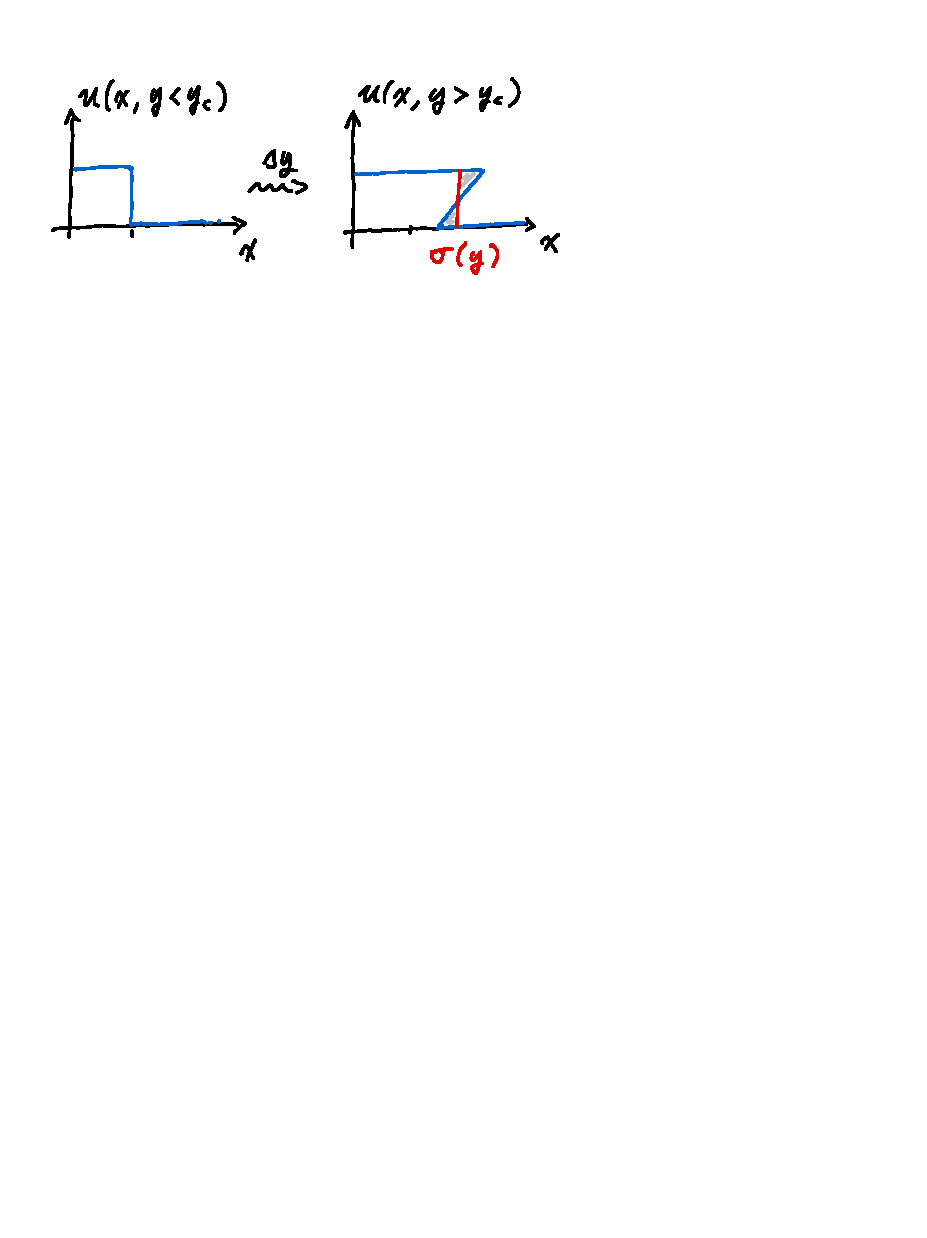
\includegraphics[
    width=.9\linewidth,
    trim=20 460 160 40, clip
  ]{figures/shockwave}
  \caption{
    \label{fig:shockwave}
    Shock wave. When the characteristic curves cross the function becomes
    multivalued. The multivalued region is replaced by a \emph{shock}
    $\sigma(y)$ which is placed such that the two gray regions have the same
    area.
  }
\end{figure}

Geometrically, the shocks are where the characteristic curves meet.
Intuitively this is a problem because the method of characteristics propagates
an information from the initial curve, and at the shock two different
information have propagated to that point (see Figure \ref{fig:shockwave}).

To check for the existence of a global weak solution, we enforce the
conservation of mass $M = \int_X u \,dx$ to the shock $\sigma(y)$, which
results in the following condition.

\begin{defn}[Ranikine-Huginot condition]
  For $u$ to be a solution weak solution of the conservation law
  \eqref{eqn:conservation-law} its \emph{shock waves} $\sigma(y)$ must have a
  speed of
  \[
    \frac{d\sigma}{dy} = \frac{f(u^+) - f(u^-)}{u^+ - u^-},
  \]
  where
  \[
    u^+(y) = \lim_{x \to\sigma(y)^+} u(x, y),
    \quad
    u^-(y) = \lim_{x \to\sigma(y)^-} u(x, y).
  \]
\end{defn}

The inverse problem to what lead to shock waves is when there is a region
where the characteristic curves \emph{diverge}, i.e. there are information to
propagate and the solution is undefined. There, the values would be
``created'' out of nothing and there are multiple solution that fit this
``hole''. Since PDEs model physical processes, a good choice is to fill in the
hole using a solution that does not break \emph{causality}, as imposed by the
next condition.

\begin{defn}[Entropy Condition]
  A weak solution satisfies the \emph{entropy condition} only if the
  characteristics enter the shock waves, and do not emerge from them. That is
  \[
    f(u^+) <
    \frac{d\sigma}{dy} = \frac{f(u^+) - f(u^-)}{u^+ - u^-}
    < f(u^-).
  \]
\end{defn}

